% -*- root: Document.tex -*-

\section{Generations}
\label{sec:generations}

As previously mentioned, \GP splits the nodes of a cluster into multiple generations, each responsible for specific types of containers and tasks.
The rationale is that, by specializing nodes for a given type of workloads, one can handle system containers whose properties are not known in advance or are dynamically evolving, while at the same time optimize the whole system's efficiency by placing the containers on the most appropriate nodes.

Along the same lines as generational garbage collectors in managed languages, \GP considers 3 generations: the nursery, the young generation, and the old generation, as illustrated in Figure~\ref{fig:generations}.

\begin{figure}[H]
  \centering
  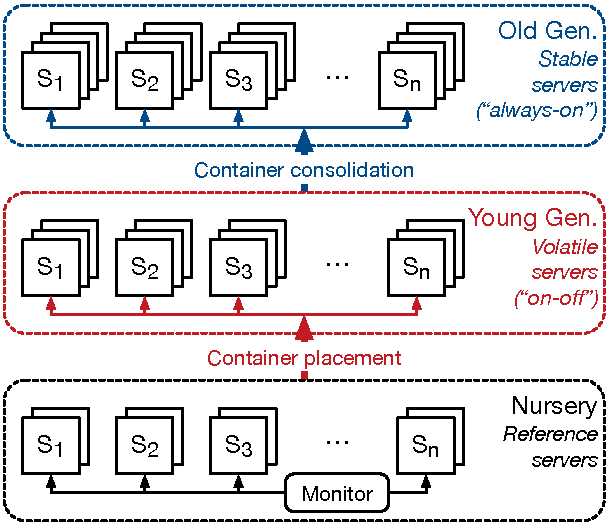
\includegraphics[width=.75\linewidth]{figures/architecture}
  \caption{\GP's different generations.}
  \label{fig:generations}
\end{figure}

% \newpage

The \emph{nursery} consists of a set of reference nodes that are representative of servers in the data center and whose properties are well understood.
A container that has not yet been profiled will first execute in the nursery.\footnote{Note that containers can skip the nursery and directly go to the next generation when previously profiled.}
During its first period of execution, \GP will monitor its resource requirements as well as its power consumption.
To that end, it leverages system-level metrics provided by \textsc{cAdvisor} (see \S\ref{sec:monitoring}) and power information from \textsc{BitWatts}~\cite{DBLP:conf/eurosys/ColmantKFHRS15}.
This observation phase allows \GP to establish a profile for the container.

Once a container's properties are known, and assuming that it did not complete its execution, it is moved to the \emph{young generation} (``placement'' phase) on a server that has sufficient resources available considering the container's specific requirements (CPU, memory, network, etc.).
The young generation hosts containers that have recently started their execution and whose lifetime is still unknown.
If the container survives long enough, it moves to the next generation.
The reasoning behind this placement strategy is that, similarly to in-memory data objects, a significant portion of the containers are expected to have a short lifetime.\footnote{We assess this statement in Section~\ref{sec:evaluation}.}
Furthermore, as the young generation is the most exposed to load variations (\textit{e.g.}, when many new containers are simultaneously launched), it will provide mechanisms for elastically scaling up and down, according to demand.
In particular, nodes can be completely turned off during periods of low load in order to considerably reduce the energy consumption of the cluster.

Finally, the \emph{old generation} consists of stable and power-efficient servers that host the long-running containers.
The placement of containers on the nodes (``consolidation'' phase) is performed in such a way that they occupy the minimum number of servers in order to optimize resource and power usage, as motivated in \S\ref{chap:motivation}.
Barring important workload variations, containers do not need to migrate further once they are on an old generation node.

The actual monitoring and scheduling operations that drive the migrations between generations are described in \S\ref{sec:monitoring} and \S\ref{sec:scheduling}.
